\documentclass[a4paper,12pt]{article}
\usepackage[T1]{fontenc}
\PassOptionsToPackage{defaults=hu-min}{magyar.ldf}
\usepackage[magyar]{babel}
	 \usepackage{graphicx, caption, url, multicol, xcolor}
	 \DeclareCaptionType{diagram} [diagram]
	 \footnotestyle{rule=fourth}
	 
	 %\setlength{\columnsep}{15mm}
	 %\setlength{\columnseprule}{0.4pt}
	 \colorlet{sargaszold}{green!30!yellow}
	 \definecolor{macibarna}{RGB}{128, 64, 0}
\begin{document}
	
	\Az{\ref{fig-diagram}}.~diagramon\footnote{Forrás: \url{https://tomacstibor.uni-eszterhazy.hu/tananyagok/diagram.pdf}} az elmúlt év vizsgajegyeinek eloszlását láthatjuk.
	\begin{diagram} [ht!]
		\centering
		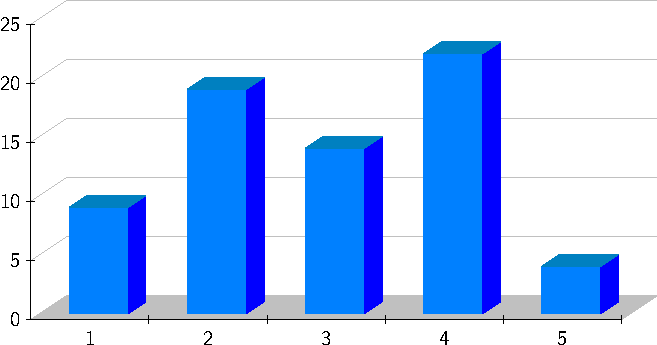
\includegraphics[width=8cm] {diagram}
		\caption{Tanulmányi eredmények 2011-ben}
		\label{fig-diagram}
	\end{diagram}
	
	Egy példa a dobozok használatára:
	
	 \begin{center}
	 	\fbox{\parbox{10cm}{Ez egy 10\,cm széles doboz, ami kapott még egy keretet
	 			is, majd középre helyeztük.
	 			
	 			Ez a doboz természetesen csak a gyakorlás kedvéért készült, sok értelme nincs.}}
	 \end{center}
	 
	 A következőkben egy kéthasábos szedést láthatunk.
	 
	 \begin{multicols}{2}
	 	A hosszúság, terület, térfogat, ívhossz, felszín, egyszerű alakzatokra
	 	már az ókori görögök által definiáltak
	 	és számolhatóak voltak.
	 	
	 	A sokszögek területének és a poliéderek térfogatának fogalmát először
	 	\textsc{Peano} és \textsc{Jordan} terjesztették ki a
	 	sík illetve a tér részhalmazainak egy
	 	nagyobb rendszerére a XIX.~század
	 	végén. Eszerint egy síkbeli korlátos
	 	halmaz külső mértéke legyen az őt lefedő véges sok sokszögből álló alakzatok területének pontos alsó korlátja, belső mértéke pedig a benne fekvő véges sok sokszögből álló alakzatok területének pontos felső korlátja.
	 	Ha ezek egyenlőek, akkor a halmazt
	 	mérhetőnek, ezen közös értéket pedig
	 	a halmaz mértékének nevezzük. Térfogat esetén hasonló az eljárás.
	 	
	 	Ez a mértékfogalom egyszerű, de
	 	az integrálás céljára nem megfelelő.
	 	Az általánosítás területén a fő lépést
	 	\textsc{Lebesgue} tette meg a XX.~század
	 	elején. Az általa alkotott mérték és
	 	integrál előnye a nagyobb általánosság, az integrál és a határátmenet felcserélhetősége.	 	
	 \end{multicols}
	 {\color{blue}30\,\% zöldhöz 70\,\% sárgát keverve a következő színt kapjuk: {\color{green!30!yellow}\rule{10mm}{3mm}} Az előző színt kereszteljük \texttt{sargaszold} névre: {\color{sargaszold}\rule{10mm}{3mm}} Definiáljon \texttt{macibarna} nevű színt, melynek RGB kódja 128, 64, 0: {\color{macibarna}\rule{10mm}{3mm}}}
	 
	 
\end{document}
